% !TEX program = xelatex
\documentclass[12pt,a4paper]{ctexart}

% === 页面设置 ===
\usepackage[top=2.5cm, bottom=2.5cm, left=2.5cm, right=2.5cm]{geometry}
\usepackage{amsmath}
\usepackage{graphicx}
\usepackage{float}
\usepackage{booktabs}
\usepackage{hyperref}
\usepackage{enumitem}
\usepackage{caption}
\usepackage{subcaption}
\usepackage{fancyhdr}
\usepackage{lastpage}
\usepackage[table]{xcolor}
\usepackage{listings}
\usepackage{tikz}

\setlength{\headheight}{14pt}
\addtolength{\topmargin}{-2pt}

\hypersetup{
    colorlinks=true,
    linkcolor=blue,
    urlcolor=blue,
    citecolor=blue,
}

\pagestyle{fancy}
\fancyhf{}
\fancyhead[L]{\small 巡迹作业一体平台}
\fancyhead[R]{\small 北京邮电大学 2026 年电子设计竞赛}
\fancyfoot[C]{\thepage}

\lstset{
    basicstyle=\ttfamily\small,
    breaklines=true,
    frame=single,
    columns=flexible,
}

% === 标题信息 ===
\title{{\Huge\bfseries 巡迹作业一体平台}\\[0.5cm]
       {\large 北京邮电大学 2026 年电子设计竞赛\\小车赛道题目 设计报告}}
\author{朱锦松\quad 郑洢陈\quad 杨照基}
\date{2026 年 7 月 9 日}

\begin{document}

\maketitle
\thispagestyle{empty}

\newpage
\setcounter{page}{1}

% ============================================================
\begin{abstract}
\noindent
本项目面向“巡迹作业一体平台”题目，设计并制作一套以 TI MSPM0G3507 为主控制器的轮式小车系统。系统由差速轮式底盘、非视觉巡迹模块、编码器/IMU 辅助运动控制模块、二维云台/作业执行模块（含 K230 视觉辅助定位）、多模块独立供电系统及人机交互模块组成。

小车通过 Yahboom 8 路灰度传感器识别黑色轨迹，结合编码器里程计和 MPU6050 姿态信息完成 A→B→C→D→A 自动运行，在 B 点和最终 A 点通过 MSPM0-K230 GPIO 握手协议触发视觉瞄准与激光作业，并实现了靶面正方形同步绘制功能。

本项目的开发历程体现了典型的工程实践特点：团队最初以“2+1”（自动巡迹 + 定点作业 + 同步绘制）为保底目标，在后期根据比赛完整要求通宵扩展至“3+2”（增加巡迹到靶位联动和四圈连续运行）。最终除因缺少无刷云台硬件而无法完成的动态跟随外，其余功能全部实现。开发期间经历了校区搬迁导致硬件损坏、陀螺仪到货延迟、首次参赛硬件经验不足等现实困难，但团队通过严格的模块化验证和回归测试策略，在每一阶段保持了底盘控制基线的稳定。

本项目的全部源代码、硬件文档、调试记录和设计报告均已在 GitHub 开源（\url{https://github.com/zhujs1103/er2024}），供后续参赛同学参考。

\vspace{1em}
\noindent\textbf{关键词：} 巡迹小车；MSPM0G3507；PID 控制；自动状态机；K230 视觉；编码器里程计；开源
\end{abstract}

\newpage
\tableofcontents
\newpage

% ============================================================
\section*{功能完成概况}
\addcontentsline{toc}{section}{功能完成概况}

\begin{table}[H]
\centering
\caption{评分项完成情况总览}
\begin{tabular}{@{}p{3cm}cp{3.5cm}p{4.5cm}@{}}
\toprule
\textbf{评分项} & \textbf{分值} & \textbf{完成情况} & \textbf{视频验证} \\
\midrule
自动巡迹与停车 & 20 & \textbf{已完成} & 见视频：自动巡迹与停车.mp4（完整巡迹、过弯跟踪、停车声光提示）\\
定点作业       & 20 & \textbf{已完成} & 见视频：定点作业.mp4（405nm 蓝紫色光点落在靶心区域）\\
巡迹到靶位联动 & 20 & \textbf{已完成} & 见视频：巡迹到靶位联动.mp4（A→B 停车作业→C→D→A，每点声光提示）\\
\rowcolor{gray!15}
动态跟随       & 15 & \textbf{未完成}（缺无刷云台硬件）& — \\
同步绘制       & 15 & \textbf{已完成} & 见视频：同步轨迹.mp4（靶面正方形绘制，图案清晰可辨）\\
四圈连续运行   & 10 & \textbf{已完成} & 见视频：四圈连续运行.mp4（4 圈 + 最终 A 点瞄准）\\
工程完善度     & $\sim$10 & \textbf{基本完成} & 模块独立供电、声光提示、调试接口\\
设计报告/AI 使用 & 10 & \textbf{已完成} & 本报告\\
\midrule
\textbf{合计（已实现）} & \textbf{85} & \multicolumn{2}{l}{\textbf{自动巡迹 20 + 定点 20 + 联动 20 + 同步绘制 15 + 四圈 10}}\\
\bottomrule
\end{tabular}
\end{table}

\noindent\textit{注：动态跟随（15 分）因缺少无刷云台导轨硬件，虽具备编码器/IMU 几何跟随基础但无法实物验证，为唯一未完成项。}

\newpage

% ============================================================
\section{题目要求分析}

\subsection{任务概述}
设计制作一套“巡迹作业一体平台”，由轮式小车底盘、巡迹控制模块和云台/机械臂作业模块组成。小车须在指定黑线场地内自动巡迹行驶，并在指定位置完成对目标靶的定点指向或标记动作。

\subsection{场地与目标靶}
\begin{itemize}[nosep]
    \item 场地尺寸：不小于 $220\times120$\,cm，白色哑光平面
    \item 轨迹：两段直线/虚线 + 两段对称半圆弧，线宽 $1.8\pm0.2$\,cm
    \item 关键点：A、B、C、D 四个（AB 参考长度约 100\,cm，半圆半径约 40\,cm）
    \item 目标靶：AB 段外侧 50\,cm，靶面与 AB 平行，高度 $\leq 50$\,cm，A4 靶面含靶心和同心圆
\end{itemize}

\subsection{硬约束}
\begin{itemize}[nosep]
    \item 外形尺寸 $\leq 25\times15\times25$\,cm
    \item 底盘轮式（禁履带、麦克纳姆轮）
    \item 主控必须为 TI 芯片
    \item 小车路径识别和目标作业不得依赖摄像头（K230 等视觉模块仅可用作执行器末端辅助定位）
    \item 云台/机械臂须独立电源控制
\end{itemize}

\subsection{基本要求（共 60 分）}
\begin{enumerate}[nosep]
    \item \textbf{自动巡迹}（20 分）：A 点出发，一圈回 A 停车，声光提示，$\leq 30$\,s
    \item \textbf{定点瞄准}（20 分）：指定位置启动后 5\,s 内对准靶心
    \item \textbf{巡迹到靶位联动}（20 分）：A→B（停车作业）→C→D→A，每点声光提示，$\leq 40$\,s
    \item \textbf{工程训练项}：模块独立上电测试，按键/串口设置参数
\end{enumerate}

\subsection{发挥要求（共 55 分）}
\begin{enumerate}[nosep]
    \item \textbf{动态跟随}（15 分）：行驶中云台持续对准目标靶
    \item \textbf{同步绘制}（15 分）：静止时在靶面绘制清晰图案
    \item \textbf{四圈连续运行}（10 分）：4 圈 + 一次完整瞄准
    \item \textbf{工程完善度}（10 分）：走线、结构强度、维护便捷、供电隔离、急停、故障恢复
\end{enumerate}
设计报告及 AI 使用说明另占 10 分。

% ============================================================
\section{总体方案}

作品采用模块化分层结构。\textbf{下层}为电池、N520 编码器电机和 8 路灰度传感器，\textbf{中层}为 MSPM0G3507 天猛星开发板、TB6612 电机驱动、LM2596 稳压模块与人机交互模块，\textbf{上层}为二维舵机云台与 K230 视觉模块。整体结构便于分别调试底盘巡迹和云台指向，各模块通过独立电源供电，调试时可单独断电任一模块而不影响其余部分。

\begin{figure}[H]
    \centering
    \begin{subfigure}[b]{0.48\textwidth}
        \centering
        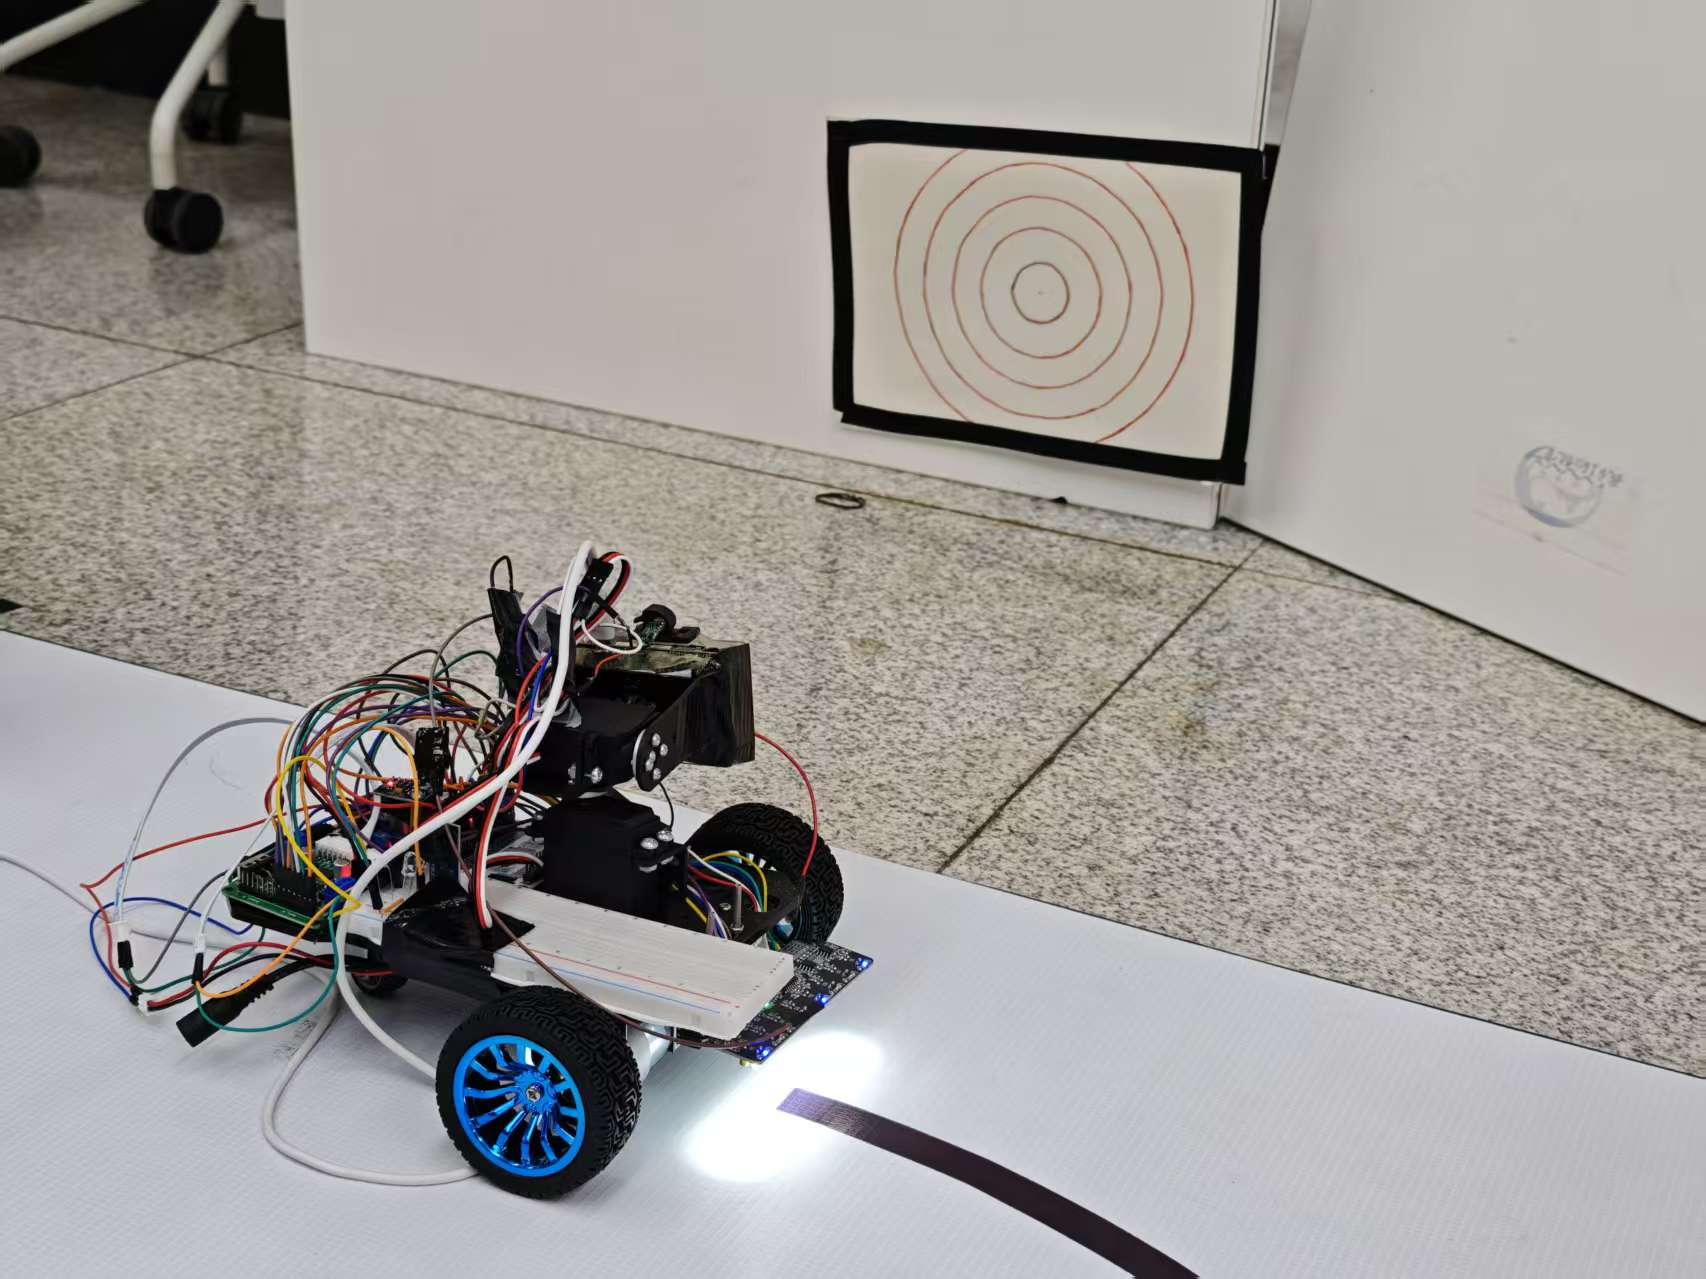
\includegraphics[width=\textwidth]{photos/01.jpg}
    \end{subfigure}
    \hfill
    \begin{subfigure}[b]{0.48\textwidth}
        \centering
        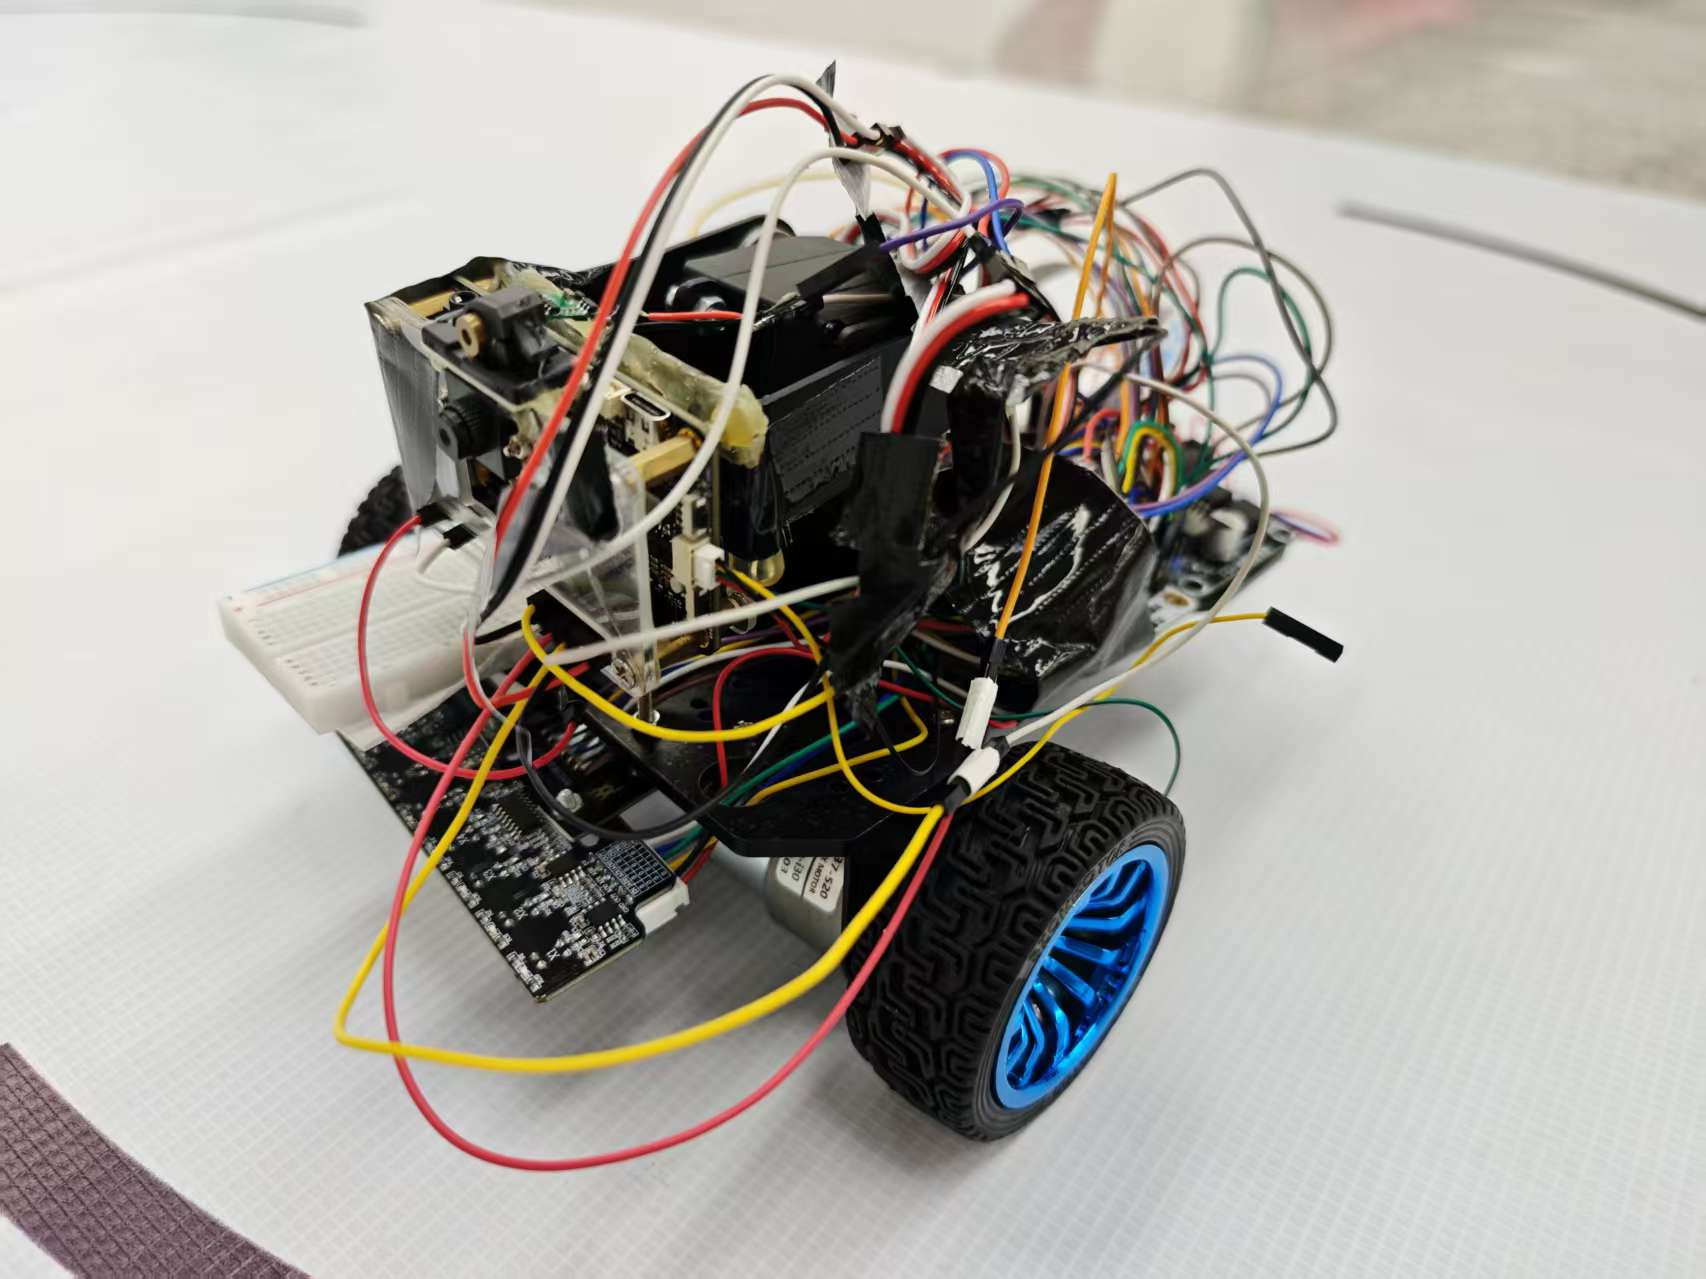
\includegraphics[width=\textwidth]{photos/02.jpg}
    \end{subfigure}
    \caption{小车整体外观}
    \label{fig:overview}
\end{figure}

% ============================================================
\section{硬件设计}

\subsection{主控制器}
选用 TI MSPM0G3507 核心开发板（嘉立创·天猛星），具备 GPIO、定时器 PWM、UART、I2C 和中断输入等资源，满足全部控制需求。调试阶段通过 USB 供电，J-Link SWD 下载程序。

\subsection{底盘与驱动}
底盘采用 2WD 轮式差速结构，电机为 12\,V 520 编码器电机，左右轮分别由 TB6612FNG 双通道模块驱动。停车时使用 TB6612 短刹车减少惯性滑行。

\begin{table}[H]
\centering
\caption{电机与编码器引脚映射}
\begin{tabular}{@{}ll@{}}
\toprule
\textbf{功能} & \textbf{引脚} \\
\midrule
左/右电机 PWM   & PA8、PA9 \\
电机方向控制    & PA16、PA21、PA22、PA23 \\
电机待机控制    & PB20 \\
左编码器 A/B    & PB17、PB18 \\
右编码器 A/B    & PB24、PB25 \\
\bottomrule
\end{tabular}
\end{table}

\subsection{巡迹传感器}
采用 Yahboom YB-MYX05-V1.0 8 路灰度传感器。该传感器为 3 位地址（AD0/AD1/AD2）选择 + 1 路 OUT 输出的复用结构。实测：白色/亮处输出 0，黑色/暗处输出 1，OUT 高电平约 3.3\,V，可直接接入 MSPM0G3507 GPIO。

\begin{table}[H]
\centering
\caption{灰度传感器引脚映射}
\begin{tabular}{@{}ll@{}}
\toprule
\textbf{传感器信号} & \textbf{MSPM0 引脚} \\
\midrule
AD0 & PA26 \\
AD1 & PA27 \\
AD2 & PA24 \\
OUT & PA25 \\
\bottomrule
\end{tabular}
\end{table}

固件将 8 个通道采样为 8 位线状态，根据黑色通道数量和位置计算加权误差：中心通道检测到黑线时误差接近 0；线偏右时误差为正，控制器提高左轮速度；线偏左时误差为负，控制器降低左轮速度。

\subsection{IMU 与白区直行}
采用 MPU6050/GY-521 模块，通过 I2C 连接主控（SCL→PB2, SDA→PB3）。启动自动模式前执行静止状态下陀螺仪 Z 轴零偏校准。白区直行时结合编码器差值和 yaw 偏差进行修正，使小车在 AB、CD 段保持直行。

\subsection{云台与执行模块}
采用二维 PWM 舵机云台（15\,kg 级），末端安装 405\,nm 蓝紫色可调焦激光模块。激光光点作为指向标记，云台通过 K230 视觉反馈实现闭环瞄准。云台使用独立 5--6\,V 高电流电源供电，与主控仅共地。激光通过 MOSFET/负载开关控制，固件默认关闭，急停和故障状态下强制关断。该设计满足题目“独立电源控制”要求。

\begin{figure}[H]
    \centering
    \begin{subfigure}[b]{0.3\textwidth}
        \centering
        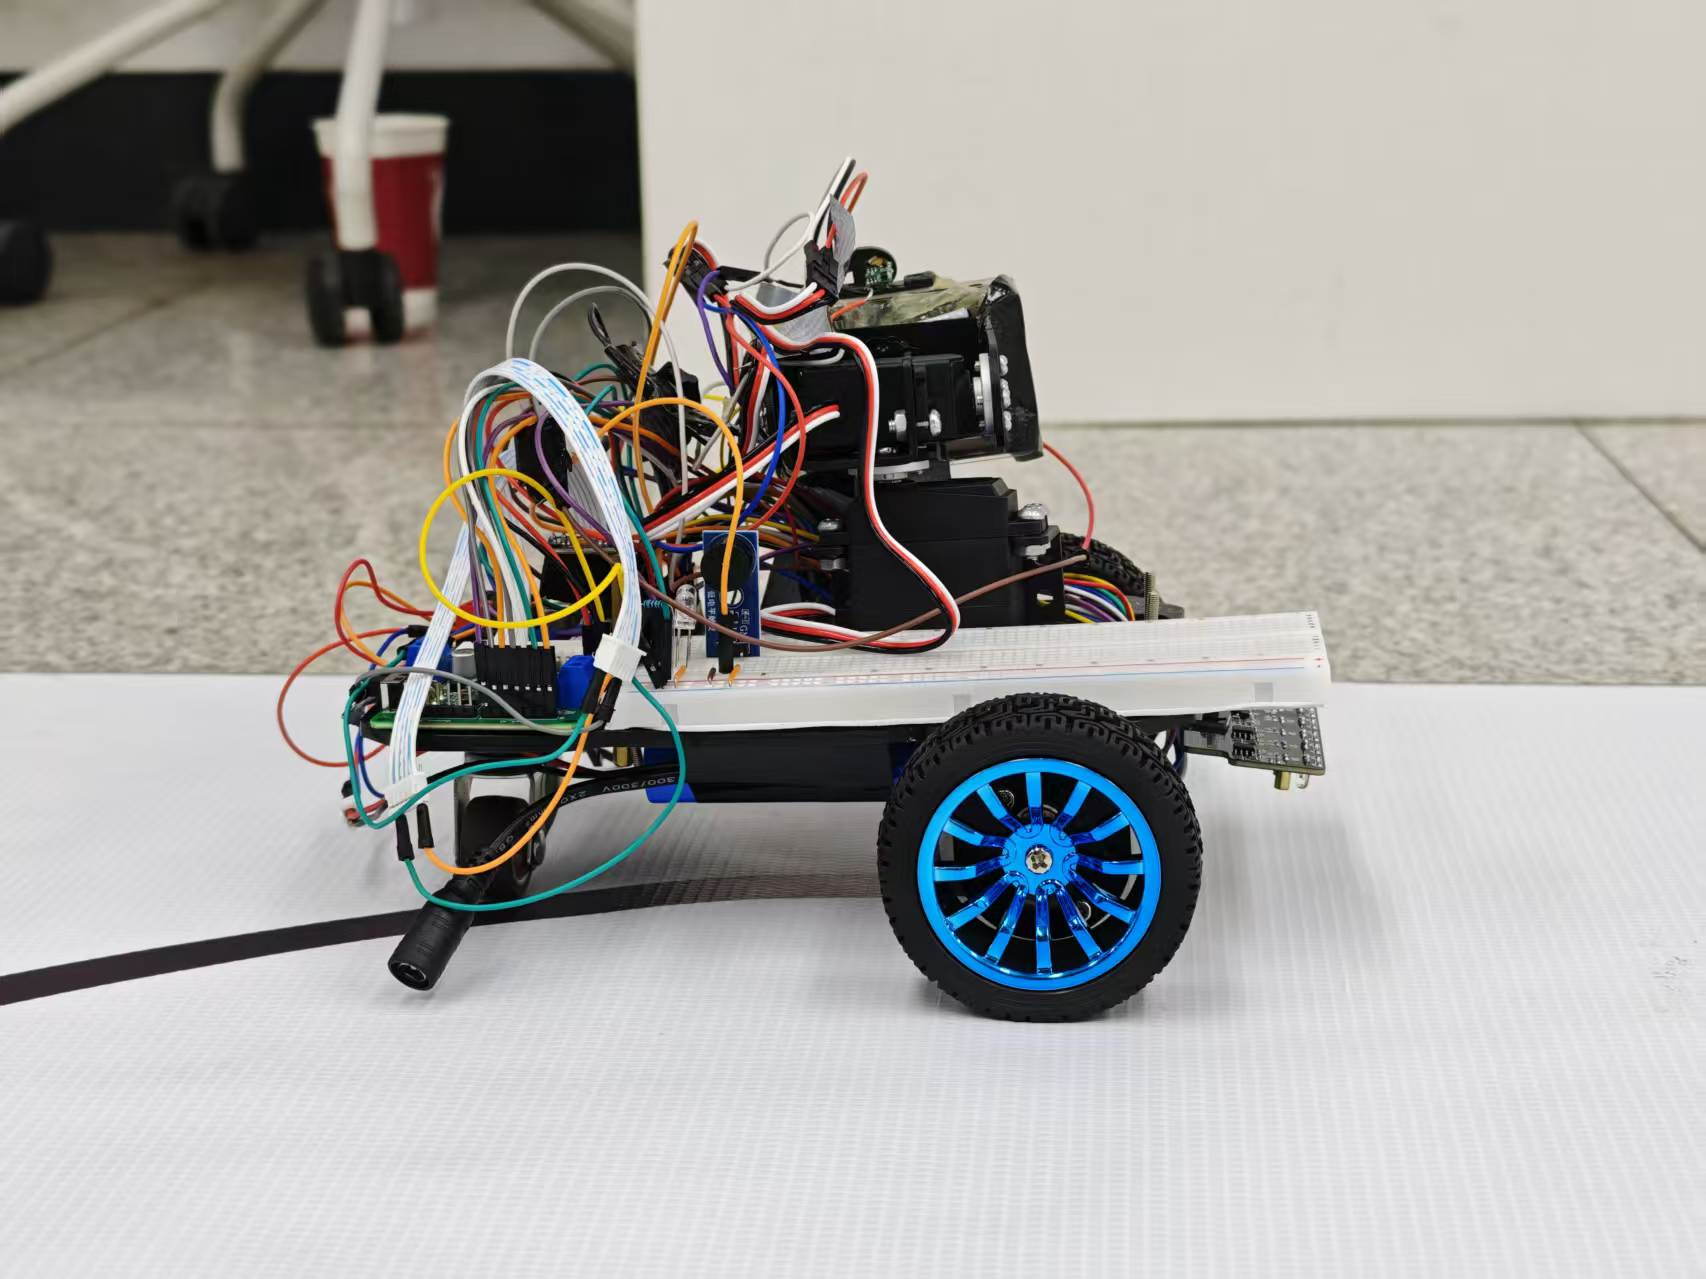
\includegraphics[width=\textwidth]{photos/03.jpg}
    \end{subfigure}
    \hfill
    \begin{subfigure}[b]{0.3\textwidth}
        \centering
        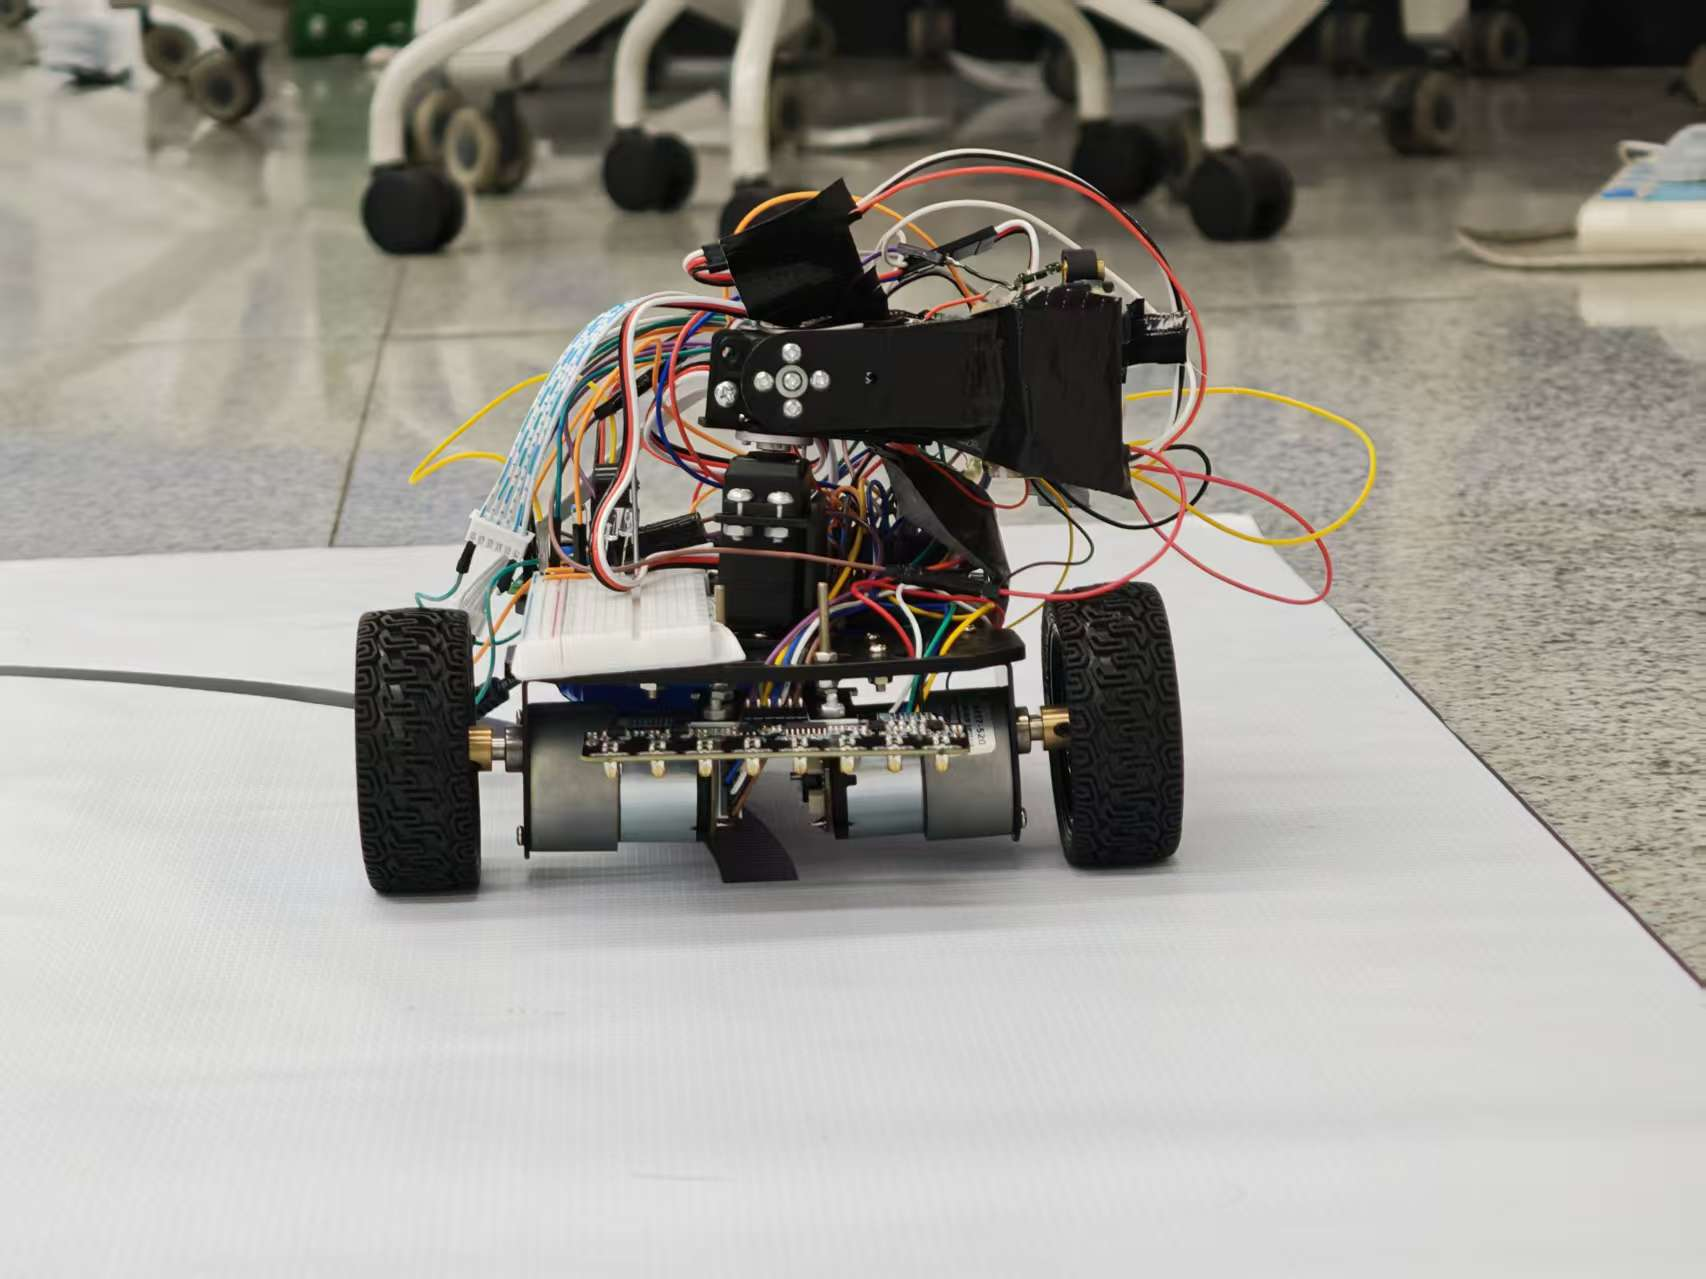
\includegraphics[width=\textwidth]{photos/04.jpg}
    \end{subfigure}
    \hfill
    \begin{subfigure}[b]{0.3\textwidth}
        \centering
        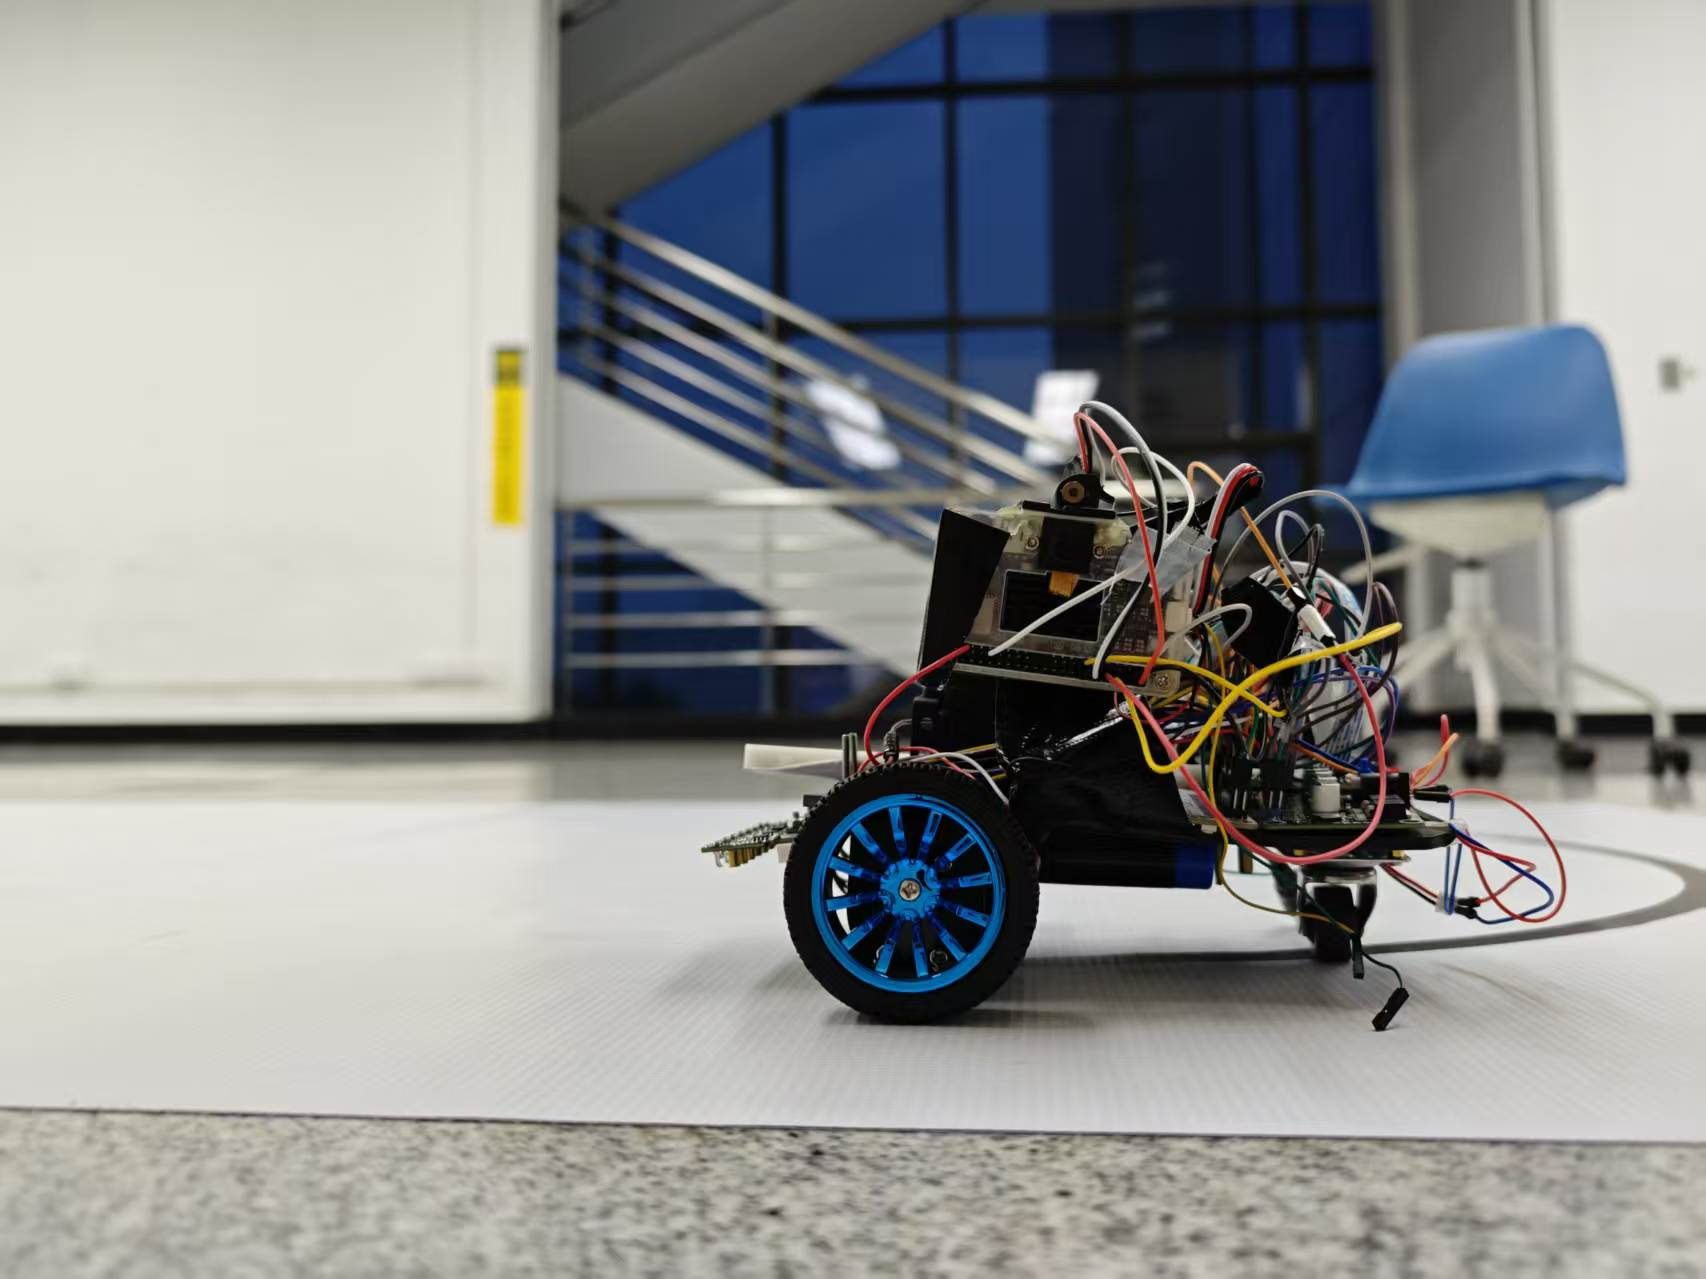
\includegraphics[width=\textwidth]{photos/05.jpg}
    \end{subfigure}
    \caption{小车多角度视图（含云台、传感器和驱动模块）}
    \label{fig:multi-angle}
\end{figure}

\subsection{人机交互}
\begin{itemize}[nosep]
    \item \textbf{UART 串口}（115200-8N1）：查看遥测数据，调整模式和参数
    \item \textbf{B21 按键}（PB21）：3\,s 倒计时启动 $\rightarrow$ 静止 IMU 校准 $\rightarrow$ 自动 Q 模式（四圈+瞄准），可按第二次取消
    \item \textbf{声光提示}：PA2 有源低电平蜂鸣器 + PA14 外部 LED + PB22 板载 LED
\end{itemize}

\subsection{供电架构}
系统采用多电源模块独立供电方案，按主控、传感器、电机驱动、云台舵机和执行光源分模块供电。调试时可单独拔掉任一模块的 VCC/GND 而不影响其他模块运行。所有模块只共享信号地，有效隔离电机和舵机大电流对主控的干扰。

% ============================================================
\section{软件设计}

\subsection{软件架构}
固件基于 TI DriverLib/SysConfig 和 Keil 工程开发（工程路径：\texttt{firmware/abcd\_four\_lap\_finish\_aim/}），主要模块包括：

\begin{enumerate}[nosep]
    \item GPIO、PWM、UART、I2C 和中断初始化
    \item 灰度传感器复用采样与 8 位线位置误差计算
    \item 左右轮 PWM 输出、方向控制和 TB6612 短刹车控制
    \item 左右编码器 GPIO 中断计数与逻辑方向修正
    \item MPU6050 初始化、gyroZ 零偏校准和 yaw 积分
    \item 巡线 PD 控制、白区直行控制和 ABCD 自动状态机
    \item 串口命令解析、遥测输出、按键消抖和声光提示
    \item K230 GPIO 握手通信（START/DONE 信号）
\end{enumerate}

\subsection{巡线 PD 控制}
巡线以 20\,ms 为控制周期。传感器读取 8 位状态后判断 OK/LOST/FULL 三类：正常黑线为 OK，全白为 LOST（容忍 300\,ms 后刹车），全黑为 FULL（立即刹车）。正常情况下计算加权误差，PD 控制生成转向修正量：

\[
\text{correction} = K_p \cdot \text{error} + K_d \cdot (\text{error} - \text{last\_error})
\]
\[
\text{left\_pwm} = \text{base} + \text{correction},\quad
\text{right\_pwm} = \text{base} - \text{correction}
\]

\begin{table}[H]
\centering
\caption{巡线 PD 参数}
\begin{tabular}{@{}lc@{}}
\toprule
\textbf{参数} & \textbf{值} \\
\midrule
控制周期 & 20\,ms \\
基准速度 base & 180/1000 \\
$K_p$ & 55 \\
$K_i$ & 0 \\
$K_d$ & 35 \\
转向限幅 & 240/1000 \\
\bottomrule
\end{tabular}
\end{table}

经地面实测，小车能够稳定跟随黑线运动。该模式也是后续 BC、DA 圆弧控制的基础。

\subsection{白区直行控制}
白区直行用于 AB 和 CD 段。传感器在白区读数为全白，不能直接提供横向误差，因此采用三重修正：
\begin{enumerate}[nosep]
    \item \textbf{编码器速度项}：比较最近一个控制周期左右轮增量，补偿瞬时速度差
    \item \textbf{编码器位置项}：比较从本段起点开始的左右累计增量，补偿长期偏航
    \item \textbf{IMU 航向项}：比较当前 yaw 与目标 yaw，补偿角度偏差
\end{enumerate}

AB 白区直行目标 yaw 为 0°；CD 白区直行目标为 $-150^\circ$。通过 \texttt{F} 命令对 AB 白区进行了独立测量，黑线入口里程约为 1558--1588\,tick，与题目中 AB 约 100\,cm 的参考长度相符。

\subsubsection*{视频验证}
见视频：自动巡迹与停车.mp4。视频中小车沿右半圆、直线/虚线段、左半圆连续运行，过弯时车头始终贴合黑线，未出现明显冲出轨迹或长时间丢线。声光指示在运行与停车阶段清晰可见。

\subsection{ABCD 自动状态机与四圈循环}
自动联动模式通过 \texttt{A} 命令（单圈）、\texttt{Q} 命令（四圈+最终瞄准）或 B21 按键启动。启动前须完成 MPU6050 静止校准（\texttt{I} 命令）。

状态机流程：
\begin{center}
\texttt{AB\_STRAIGHT} $\rightarrow$ \texttt{B\_GUARD} $\rightarrow$ \texttt{BC\_LINE} $\rightarrow$ \texttt{C\_ALIGN} $\rightarrow$ \texttt{CD\_STRAIGHT} $\rightarrow$ \texttt{D\_GUARD} $\rightarrow$ \texttt{DA\_LINE}
\end{center}

\begin{table}[H]
\centering
\caption{ABCD 状态功能表}
\begin{tabular}{@{}lp{9cm}@{}}
\toprule
\textbf{状态} & \textbf{功能} \\
\midrule
AB\_STRAIGHT & 等待全白起点，编码器平衡+IMU 航向（0°）向 B 前进，里程 1200--1900\,tick 内寻黑线 \\
B\_GUARD     & B 点短保护（15--45\,tick），防止边缘黑线造成过大 PID 修正 \\
BC\_LINE      & PD 巡线跟踪 B→C 圆弧，出口：里程 1500--2600\,tick + 连续丢线确认 3 周期 \\
C\_ALIGN      & 纯 IMU 航向对齐 CD 目标（$-150^\circ$），编码器平衡关闭 \\
CD\_STRAIGHT  & 白区直行向 D 前进，航向 $-150^\circ$ \\
D\_GUARD      & D 点入口保护（同 B 点逻辑） \\
DA\_LINE      & PD 巡线跟踪 D→A 圆弧 \\
\bottomrule
\end{tabular}
\end{table}

\subsubsection*{四圈循环逻辑}
DA 弧线出口确认后，若已完成圈数 $<$ 目标圈数（Q 模式为 4），进入 \texttt{A\_NEXT\_ALIGN} 状态，以 $-303^\circ$ 航向完成下一圈 AB 入口对准，随后将 yaw 归零并重新进入 \texttt{AB\_STRAIGHT}。每圈 yaw 独立不累积，避免角度溢出。

\subsubsection*{最终瞄准}
第 4 圈 DA 出口后进入 \texttt{A\_ALIGN}（最多 150\,tick 短对准），随后无条件进入 \texttt{A\_FINISH\_WORK}，通过 PB11 拉高 START 触发 K230 视觉瞄准。MSPM0 等待 PB14 DONE 信号稳定 40\,ms 确认完成；15\,s 超时判定失败。

\begin{table}[H]
\centering
\caption{四圈关键参数（现场调参确定）}
\begin{tabular}{@{}lcl@{}}
\toprule
\textbf{参数} & \textbf{值} & \textbf{说明} \\
\midrule
CD\_YAW   & $-15000$ ($-150^\circ$) & CD 直行航向，从 $-153^\circ$ 微调解决 D 点右侧偏移 \\
NEXT\_AB  & $-30300$ ($-303^\circ$) & 圈间 AB 重入航向（$-325^\circ$ 偏右，$-300^\circ$ 偏左）\\
AIM       & $-36000$ ($-360^\circ$) & 最终 A 点瞄准航向 \\
CORR\_MAX & 40                    & IMU 修正上限 \\
\bottomrule
\end{tabular}
\end{table}

\subsection{MSPM0-K230 握手协议与视觉作业}

MSPM0 与 K230 视觉模块通过 3.3\,V GPIO 直连通信：

\begin{table}[H]
\centering
\caption{MSPM0-K230 握手引脚}
\begin{tabular}{@{}lll@{}}
\toprule
\textbf{MSPM0} & \textbf{K230} & \textbf{方向/含义} \\
\midrule
PB11 & GPIO03 & MSPM0→K230：START，高电平触发瞄准 \\
PB14 & GPIO04 & K230→MSPM0：DONE，高电平表示瞄准+激光完成 \\
GND  & GND    & 共地 \\
\bottomrule
\end{tabular}
\end{table}

K230 运行 MicroPython 脚本，工作流程为：
\begin{enumerate}[nosep]
    \item 等待 START 高电平
    \item 灰度 blob 检测黑色靶框（阈值 0--35，宽 $\geq$ 80\,px，高 $\geq$ 50\,px）
    \item 二维舵机（PWM3/PWM4，50\,Hz）迭代逼近靶心（死区 $\pm$15\,px）
    \item 瞄准稳定 5 帧后激光点亮 3\,s
    \item 拉高 DONE
    \item 等待 START 低电平后复位
\end{enumerate}

\subsubsection*{同步绘制功能}
另一 K230 脚本实现正方形绘制。瞄准稳定后，舵机按预设正方形路径分段移动（每边 25 步，尺寸参数 \texttt{DRAW\_SIZE\_X/Y=0.15}，整体左移 \texttt{SQUARE\_LEFT\_OFFSET=0.45}），405nm 蓝紫色激光持续点亮形成清晰轨迹。

\subsubsection*{视频验证}
见视频：定点作业.mp4（405nm 蓝紫色光点落在同心圆靶中心区域附近，验证定点作业功能）及同步轨迹.mp4（靶面正方形图案清晰可辨，与预设设计相符）。

\subsection{串口命令体系}
\begin{table}[H]
\centering
\caption{主要串口命令}
\begin{tabular}{@{}ll@{}}
\toprule
\textbf{命令} & \textbf{作用} \\
\midrule
\texttt{A/a} & 启动单圈 ABCD 自动状态机 \\
\texttt{Q/q} & 启动四圈 + 最终 A 点 K230 瞄准 \\
\texttt{T/t} & 启动单圈 + B 点视觉瞄准（旧模式） \\
\texttt{F}   & 白区直行到黑线的单段测试 \\
\texttt{G}   & 连续黑线巡迹测试 \\
\texttt{I}   & MPU6050 初始化 + gyroZ 零偏校准 \\
\texttt{Y/y} & 独立 IMU 辅助直行测试 \\
\texttt{+/-} & 调整基准速度 \\
\texttt{p/P} & 调整 $K_p$ \\
\texttt{d/D} & 调整 $K_d$ \\
\texttt{b}   & 短刹车 \\
\texttt{x}   & 空转停止 \\
\texttt{?}   & 打印帮助和当前参数 \\
\bottomrule
\end{tabular}
\end{table}

% ============================================================
\section{开发历程与调试}

本章以时间顺序记录项目的完整开发过程，重点展示团队在硬件限制、经验不足和时间压力下如何通过分阶段验证和迭代调试逐步推进。

\subsection{第一阶段：让芯片跑起来（6 月 29 日）}

首日即遇到多个工具链和硬件配置问题：

\begin{itemize}
    \item \textbf{J-Link 版本过低}：Keil 自带的 J-Link DLL V6.86 不识别 MSPM0G3507，需升级 SEGGER J-Link 至 V9.54
    \item \textbf{排线接错}：20-pin ARM 排线按颜色接线导致 SWD 连不上，最终按引脚号（1=VT, 7=DIO, 9=CLK, 15=RST）重接成功
    \item \textbf{调试器模式错误}：初始误配为 CMSIS-DAP/JTAG，正确配置为 J-Link SWD @ 100\,kHz
    \item \textbf{串口混淆}：板载 CH340 枚举为 COM9，J-Link 虚拟串口为 COM10，须使用 COM9
    \item \textbf{烧录后不运行}：需手动按 RST 复位
\end{itemize}

成功标志：Keil 编译 0 Error，J-Link SWD 检测到 \texttt{ARM CoreSight SW-DP (IDCODE 0x6BA02477)}，Flash 烧录 \texttt{Erase/Programming/Verify OK}，PB22 LED 健康闪烁。

\subsection{第二阶段：电机与编码器（6 月 30 日）}

电机驱动验证阶段暴露了多个底层硬件问题：

\begin{itemize}
    \item \textbf{左轮方向相反}：不改接线，软件中翻转 motor A/B 方向标志解决
    \item \textbf{右路驱动疑似故障}：TB6612 右通道输出异常，通过交叉验证确认模块问题后更换
    \item \textbf{编码器符号不一致}：前进时 encL 递减、encR 递增，翻转左编码器符号使两侧同向
    \item \textbf{停车滑行}：开环 PWM 停车时右轮多滑半圈，加入 TB6612 短刹车（AIN1=AIN2=BIN1=BIN2=1，PWM 满占空）
    \item \textbf{方向基准错误}：小车测试时方向拿反导致所有方向标志错位，7 月 1 日全面纠正：mSwap=1, invA=1, invB=1, sensorFlip=1, eSwap=1, eInvA=1, eInvB=1
\end{itemize}

\subsection{第三阶段：地面巡线（7 月 1 日）}

从零开始调参，通过串口遥测反复迭代：

\begin{itemize}
    \item 传感器物理位序（bit0=右, bit7=左）与逻辑帧不一致，通过 sensorFlip=1 软件翻转
    \item PD 参数从保守值起步，地面实测收敛至 base=180, $K_p$=55, $K_d$=35, $K_i$=0
    \item 全黑（0xFF）和全白（0x00）异常状态分别处理：全黑立即刹车，全白容忍 300\,ms
\end{itemize}

从 2306 行串口遥测数据提取验证：RUN 模式下误差范围 $[-300, 350]$，修正量范围 $[-182, 192]$，电机转向和传感器方向逻辑正确。

\subsection{第四阶段：ABCD 状态机——最艰难的攻坚（7 月 2 日--4 日）}

ABCD 自动联动是本项目开发中最具挑战性的阶段，经历了多次失败和完全重写：

\begin{enumerate}
    \item \textbf{第一次 A 模式崩溃}：AB→BC 转换后立即停车（\texttt{mode=STBY, L=0, R=0}），根因是旧状态机逻辑混乱，决心完全重写
    \item \textbf{重写后 BC 弧线过早退出}：\texttt{arc lost early at segOdom=1888}，放宽出口窗口至 1500--2600\,tick
    \item \textbf{CD 直行里程计混乱}：编码器 reset 和 odom 清零的时序 bug 导致 CD 段超时，修正为强制清零后再启动
    \item \textbf{B 点入口错过}：3 次采样确认过于保守，改为 1 次采样即触发
    \item \textbf{UART 日志阻塞控制}：9600\,baud 下状态切换日志延迟了电机指令，改为先发驱动指令再打印紧凑日志，并将波特率提升至 115200
    \item \textbf{C 点假触发}：弧线未过半就误判出口，明确不使用 yaw 角度硬判，改为里程+丢线确认
    \item \textbf{CD 航向偏差迭代}：CD 直行持续偏右，经多轮现场调参：$-180^\circ \rightarrow -155^\circ \rightarrow -153^\circ \rightarrow \mathbf{-150^\circ}$
\end{enumerate}

7 月 4 日，\texttt{cd-yaw-153} 构建完成了两次完整 ABCDA 环路，标志着底盘联动达到可恢复基线。

\subsection{第五阶段：四圈 + K230 瞄准（7 月 8 日--9 日）}

在底盘联动稳定后，团队在最后阶段通宵冲刺四圈连续运行和 K230 视觉联调：

\begin{itemize}
    \item \textbf{四圈 yaw 溢出}：四圈累积 yaw 超过 $\pm450^\circ$ 上限，改为每圈 A 出口 rebase 归零
    \item \textbf{圈间 AB 入口角度}：$-325^\circ$ 偏右漏 B、$-300^\circ$ 偏左撞边，二分法收敛至 $\mathbf{-303^\circ}$
    \item \textbf{A\_ALIGN 死循环}：纯 IMU 对齐无法收敛，改为限 150\,tick 无条件进入 A\_FINISH\_WORK，精细瞄准交由 K230
    \item \textbf{K230 DONE 抖动}：GPIO 边沿抖动导致误判完成，加入 40\,ms 稳定确认窗口
    \item \textbf{SysConfig 1.28 兼容}：\texttt{initialValue=CLEARED}、UART 使用 profile 模式、MFCLK 需 clockTree 门控
\end{itemize}

\subsection{现实困难与反思}

整个开发过程并非一帆风顺，团队面临了多重现实约束：

\begin{itemize}
    \item \textbf{校区搬迁}：从沙河校区搬至本部期间，部分硬件在运输中损坏，且搬迁占用了宝贵的调试时间
    \item \textbf{硬件经验不足}：团队首次参加电子设计竞赛，在硬件选型和接线方面缺乏经验。陀螺仪（MPU6050）到货较晚，导致白区直行控制调试起步延迟
    \item \textbf{无刷云台缺失}：由于缺少无刷导轨硬件，动态跟随功能虽在软件层面具备编码器/IMU 几何跟随基础，但无法在实物上验证和演示，成为唯一未完成的功能项
    \item \textbf{策略调整与通宵冲刺}：团队初始以“2+1”（自动巡迹 + 定点作业 + 同步绘制）为保底目标。在了解到比赛完整提交要求后，连夜将目标扩展为“3+2”（增加巡迹到靶位联动和四圈连续运行），最终成功交付
\end{itemize}

这些经历让团队深刻认识到：\textbf{硬件先行、充分备件、尽早联调}是竞赛成功的关键前提。下一次参赛将在硬件准备和风险预案方面做更充分的规划。

% ============================================================
\section{工程完善度}

\subsection{模块独立上电与调试}
系统按主控、传感器、电机驱动、云台舵机和执行光源分模块供电。调试时只需拔掉对应模块的 VCC/GND 即可单独断电调试，所有模块仅共享信号地。软件层面保留 F/G/Y 等独立测试模式，使白区直行、黑线巡迹和 IMU 辅助直行可以分开回归测试，避免调试自动状态机时破坏已验证底层功能。

\subsection{安全默认状态}
固件要求电机 STBY、激光、照明和舵机输出在复位和故障状态下保持关闭。自动状态机失败、传感器异常、IMU 丢失或人工急停时，电机进入短刹车或待机状态，并通过蜂鸣器和 LED 声光提示故障类型。

\subsection{调试接口与可维护性}
硬件上预留 USB 下载口、UART 调试口、模块电源接口和公共地测试点。软件上串口 \texttt{?} 命令可实时查看全部运行参数，\texttt{+/-/p/P/d/D} 等命令支持运行中调参，无需重新编译烧录。

\begin{figure}[H]
    \centering
    \begin{subfigure}[b]{0.48\textwidth}
        \centering
        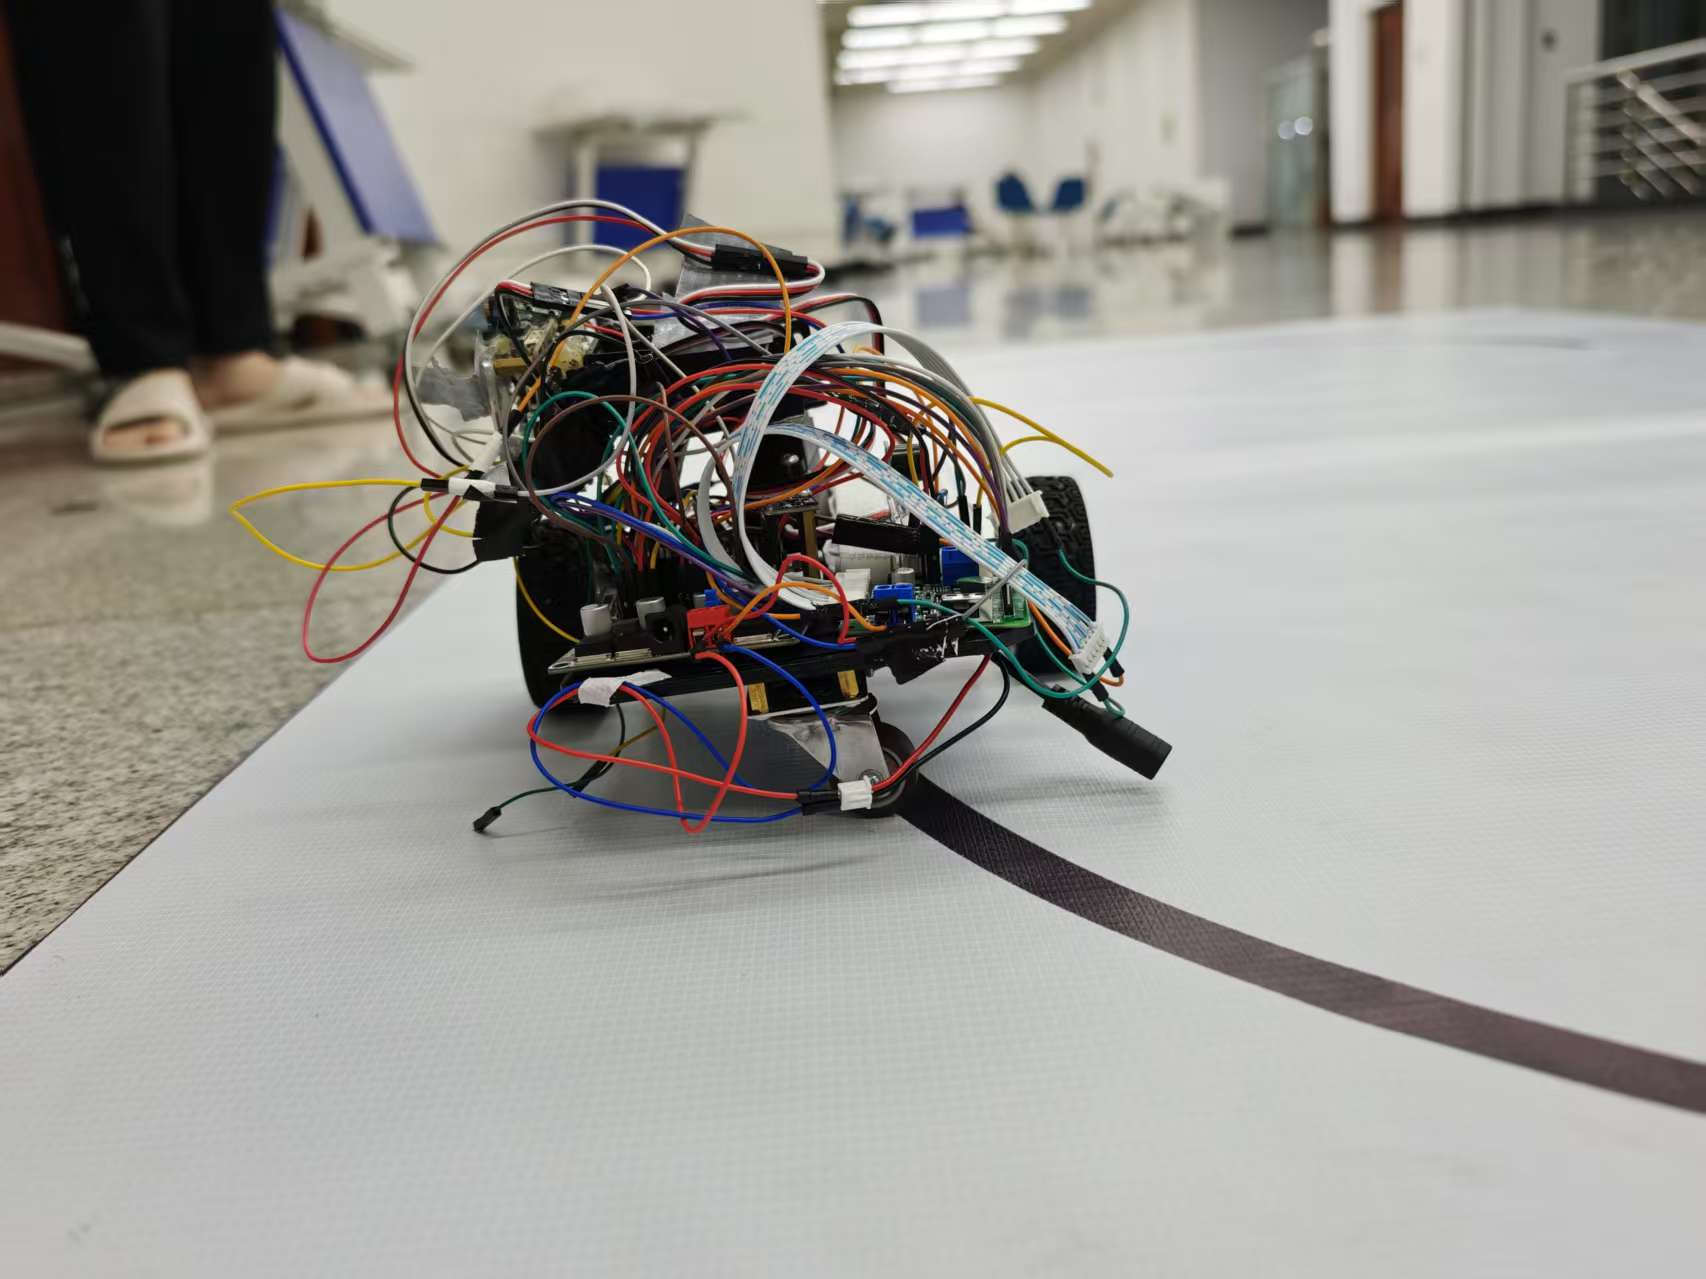
\includegraphics[width=\textwidth]{photos/06.jpg}
    \end{subfigure}
    \hfill
    \begin{subfigure}[b]{0.48\textwidth}
        \centering
        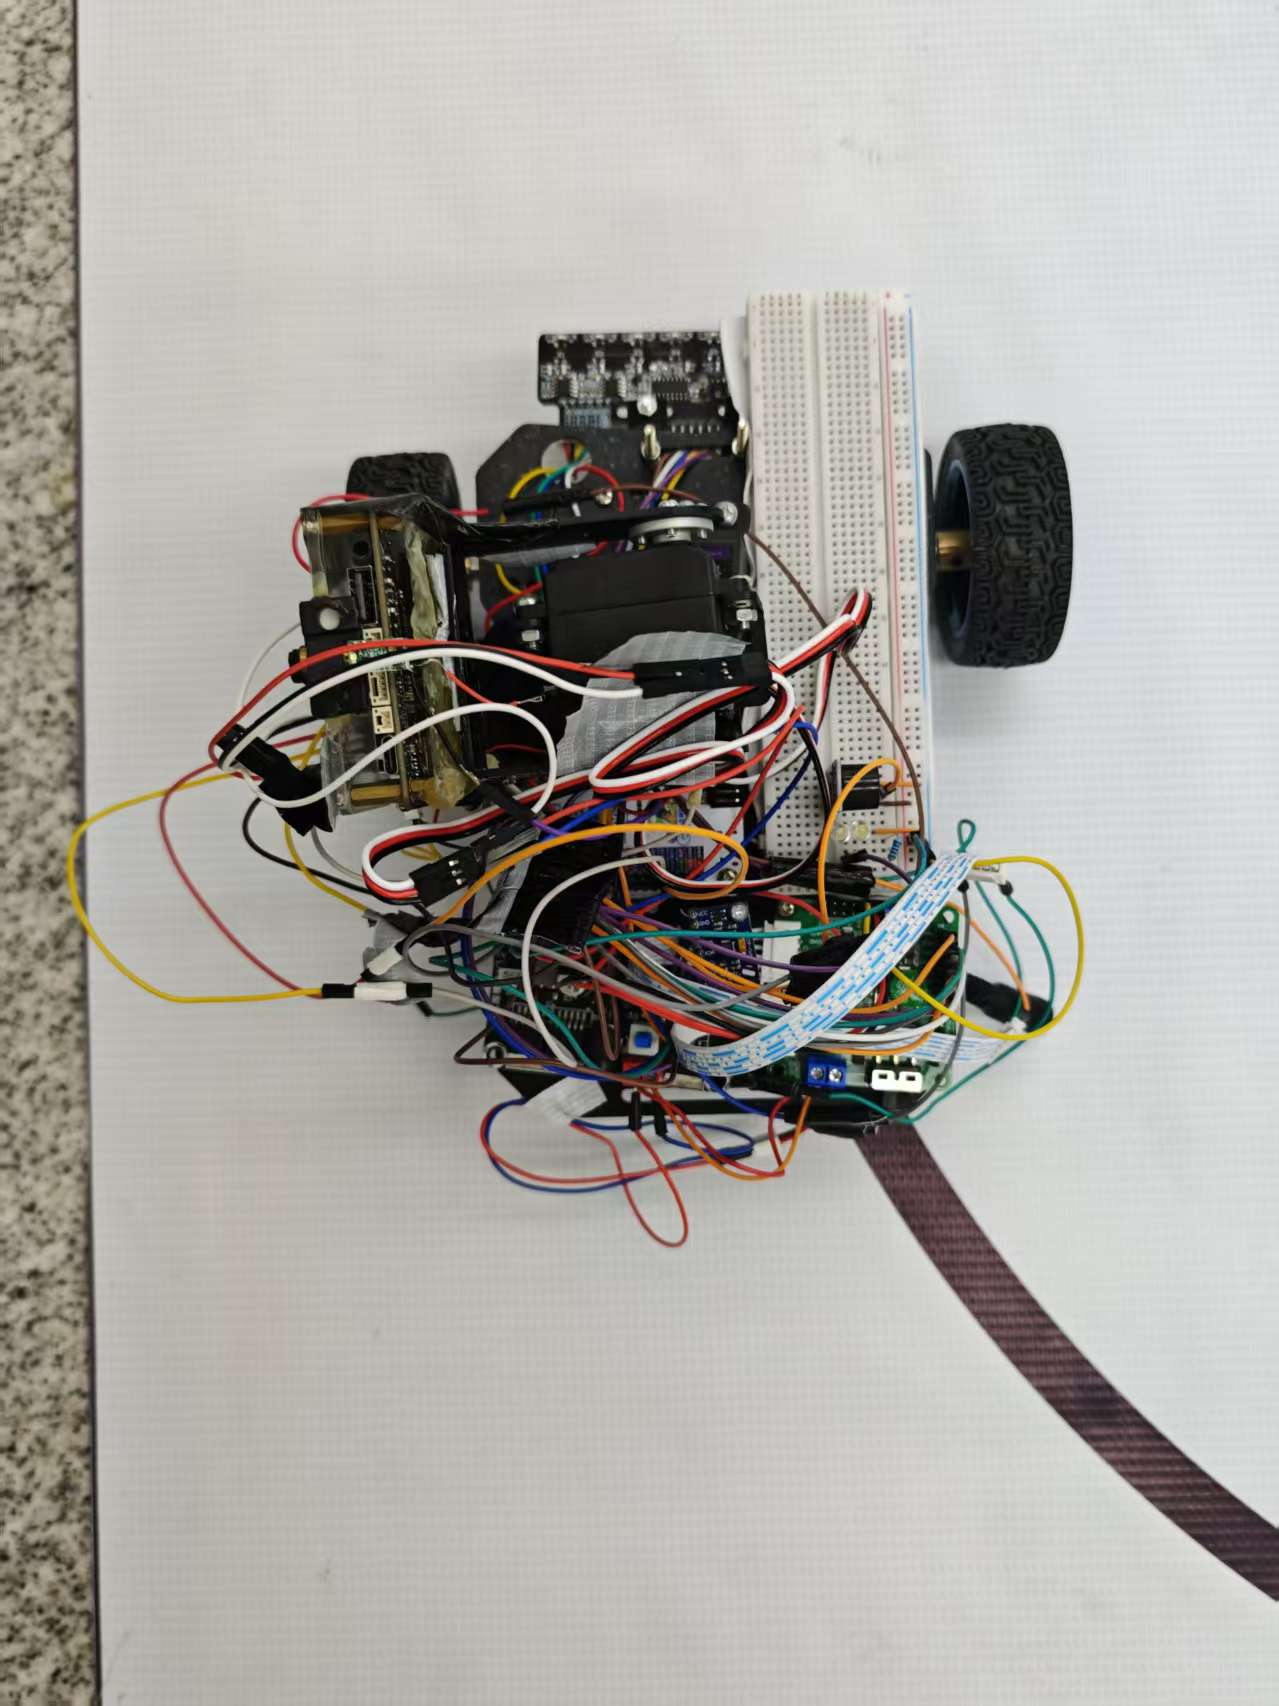
\includegraphics[width=\textwidth]{photos/07.jpg}
    \end{subfigure}
    \caption{小车细节视图（可见接线和模块布局）}
    \label{fig:detail}
\end{figure}

% ============================================================
\section{功能完成情况}

\begin{table}[H]
\centering
\caption{功能完成情况对照表}
\begin{tabular}{@{}p{3cm}cp{5.5cm}@{}}
\toprule
\textbf{评分项} & \textbf{分值} & \textbf{完成情况} \\
\midrule
自动巡迹与停车 & 20 & \textbf{已完成}。PD 巡线 + 编码器停车，现场测试通过 \\
定点作业 & 20 & \textbf{已完成}。K230 视觉瞄准 + 二维舵机 + 激光 3\,s 射击，握手协议验证通过 \\
巡迹到靶位联动 & 20 & \textbf{已完成}。ABCD 状态机完整环路，单圈/四圈模式均可运行 \\
\rowcolor{gray!15}
动态跟随 & 15 & \textbf{未完成}。因缺少无刷云台硬件，虽具备编码器/IMU 几何基础但无法实物验证 \\
同步轨迹 & 15 & \textbf{已完成}。K230 脚本实现靶面正方形绘制，参数可调 \\
四圈连续运行 & 10 & \textbf{已完成}。Q 模式四圈 + 最终瞄准，现场调参稳定 \\
工程完善度 & $\sim$10 & \textbf{基本完成}。模块独立供电、安全默认、调试接口和声光提示均已实现 \\
设计报告/AI 使用说明 & 10 & \textbf{已完成}。本报告详细说明 AI 使用过程、帮助与局限 \\
\midrule
\textbf{合计（已实现）} & \textbf{85} & \textbf{自动巡迹 20 + 定点作业 20 + 联动 20 + 同步绘制 15 + 四圈 10} \\
\bottomrule
\end{tabular}
\end{table}

\noindent\textit{注：动态跟随（15 分）因硬件限制未实现；工程完善度和设计报告得分以评审为准。}

% ============================================================
\section{项目 AI 使用说明}

\subsection{使用的工具}
本项目在需求拆解、硬件选型、文档整理、固件开发、调试分析和报告撰写过程中使用了 AI agent 工具 Codex。AI 工具不直接替代实物测试，所有涉及电气安全、引脚连接、运动效果和比赛功能的结论均通过本地资料、代码、编译或实测结果验证。

\subsection{使用方式}
\begin{enumerate}[nosep]
    \item \textbf{需求分析}：将题目 PDF 提取为文本，整理硬约束、基本要求、发挥要求和提交材料清单
    \item \textbf{硬件规划}：根据已购器件建立硬件清单，区分已知参数、未知参数和需实测的安全风险
    \item \textbf{接线与安全检查}：为各模块建立分阶段接线和上电计划，标注电平安全和供电隔离要点
    \item \textbf{固件开发}：在 Keil/SysConfig 工程中实现传感器采样、电机 PWM、编码器计数、巡线 PD、白区直行、IMU 校准、ABCD 自动状态机、四圈循环、K230 握手、声光提示和按键启动等全部逻辑
    \item \textbf{调试分析}：根据 2300+ 行串口日志分析每次失败的根本原因，区分硬件方向、电机控制、传感器识别和状态机逻辑问题
    \item \textbf{项目管理}：持续维护 roadmap、risk register、bring-up record、AI usage log 和自动调试 handoff，保证多次中断后仍能恢复上下文
    \item \textbf{报告撰写}：基于题目要求、项目文档和实测记录生成本设计报告
\end{enumerate}

\subsection{对项目的帮助}
AI 工具显著提高了需求拆解和调试记录的效率。它帮助团队把题目从自然语言转化为可执行的工程检查项，把硬件风险提前整理为上电顺序和安全默认状态，并在固件调试中保存每次失败的现象、原因和下一步测试顺序。对于 ABCD 自动状态机这类长流程问题，AI 还帮助把已验证的 F/G/Y 单项测试与自动模式隔离，减少对已通过功能的破坏。在四圈调参阶段，AI 辅助分析了 yaw 角度偏差与入口偏移的定量关系，加速了 NEXT\_AB 参数（$-325^\circ \rightarrow -303^\circ$）的收敛。

\subsection{局限性与控制措施}
AI 工具无法直接观察实物电路，也不能替代万用表测量、示波器验证、现场跑车和安全评估。它可能根据常见模块经验做出不适用于本项目具体器件的假设。因此项目采取以下控制措施：

\begin{enumerate}[nosep]
    \item 以题目原文、实物照片、模块丝印、数据手册和本地代码为依据，不凭空假设接口
    \item 所有电源、电平和电机方向先低风险验证，再接入自动控制
    \item 固件修改后进行代码检查和 Keil 编译验证，现场测试前保留已通过的 F/G/Y 回归模式
    \item 报告中对未完成或未实测功能明确说明原因（如硬件缺失），避免把设计目标写成已通过结果
\end{enumerate}

% ============================================================
\section{总结与展望}

本项目围绕比赛 85 分功能目标，完成了以 MSPM0G3507 为核心、非视觉灰度巡迹+编码器里程计+IMU 航向保持+K230 视觉辅助瞄准的巡迹作业一体平台。项目在底盘控制、自动状态机、多传感器融合和主从视觉握手等方面积累了完整的工程经验。

作为首次参加电子设计竞赛的团队，我们经历了从零搭建开发环境、逐模块验证硬件、反复重写状态机、连夜冲刺扩展功能的全过程。校区搬迁、陀螺仪延迟到货、无刷云台缺失等现实困难让我们深刻认识到\textbf{硬件准备和风险预案在竞赛中的关键作用}。这些经验将成为下一次参赛的重要基础。

本项目完整工程已开源至 GitHub：\url{https://github.com/zhujs1103/er2024}，包含固件源代码、K230 视觉脚本、硬件文档、调试记录和设计报告，欢迎交流与参考。

\vspace{1em}
\begin{center}
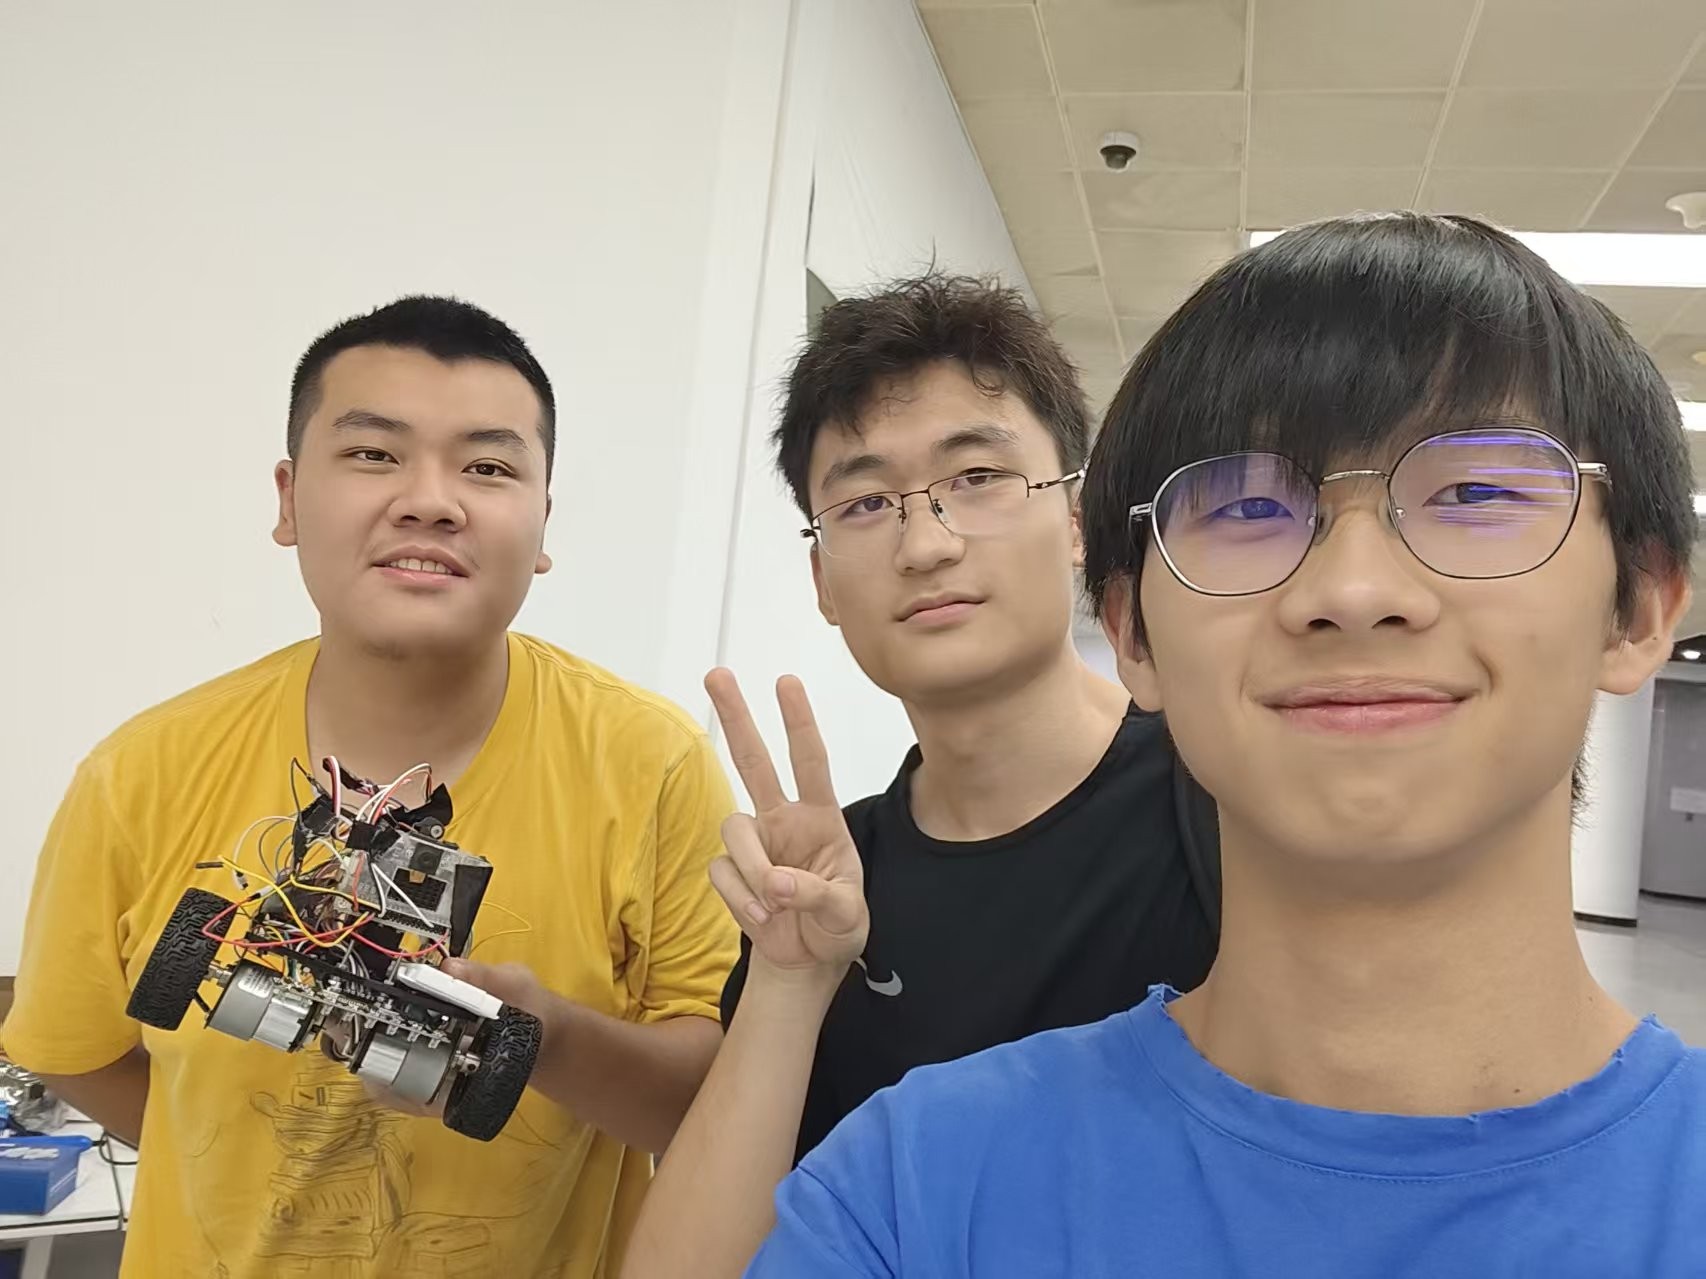
\includegraphics[width=0.55\textwidth]{photos/08_team.jpg}
\captionof{figure}{团队成员与小车合影}
\label{fig:team}
\end{center}

% ============================================================
\appendix
\section{主要项目资料来源}

\begin{table}[H]
\centering
\begin{tabular}{@{}lp{10cm}@{}}
\toprule
\textbf{资料} & \textbf{用途} \\
\midrule
\texttt{competition\_requirements/} & 题目原文、需求整理、评分策略 \\
\texttt{hardware\_docs/purchased\_hardware\_registry.md} & 已购 17 项硬件清单 \\
\texttt{hardware\_docs/assembly\_wiring\_plan.md} & 分阶段接线和安全上电方案 \\
\texttt{hardware\_docs/firmware\_integration\_matrix.md} & 各硬件模块软件接口 \\
\texttt{hardware\_docs/step5\_motor\_encoder\_bringup\_record.md} & 电机与编码器调试记录 \\
\texttt{hardware\_docs/step6\_pid\_line\_following\_bringup\_record.md} & 低速巡线验证记录 \\
\texttt{hardware\_docs/step7\_one\_lap\_encoder\_stop\_bringup\_record.md} & 白区直行与 A 模式调试记录 \\
\texttt{firmware/abcd\_four\_lap\_finish\_aim/} & 主力四圈+瞄准固件工程 \\
\texttt{vision/k230\_a\_finish\_aim\_handshake.py} & K230 瞄准握手脚本 \\
\texttt{vision/正方形[1].py} & K230 正方形绘制脚本 \\
\texttt{project\_management/ai\_usage\_log.md} & AI 使用过程记录 \\
\texttt{project\_management/roadmap.md} & 分阶段实施计划 \\
\texttt{project\_management/risk\_register.md} & 技术风险与缓解措施 \\
\bottomrule
\end{tabular}
\end{table}

\section{提交材料清单}

\begin{table}[H]
\centering
\begin{tabular}{@{}ll@{}}
\toprule
\textbf{材料} & \textbf{说明} \\
\midrule
设计报告（本文件） & LaTeX 排版，含图文和 AI 使用说明 \\
GitHub 开源仓库 & \url{https://github.com/zhujs1103/er2024}（含全部固件源码、K230 脚本、硬件文档和调试记录） \\
外观照片 & \texttt{photos/} 共 8 张 \\
演示视频 & 5 个：自动巡迹与停车、定点作业、巡迹到靶位联动、同步轨迹、四圈连续运行\\
\bottomrule
\end{tabular}
\end{table}

\end{document}
